%Qué resultados obtuvimos del análisis en cuestión. Acá vamos a poner qué palabras fueron significativas, dónde lo fueron, y demás.

% Distribucion de entropía vs frecuencia  
% Distribucion de frecuencias de las palabras
% Distr entropia
% de valor de la inf. a partir de los 5000 se ve que se estanca (graficar hasta 10**5)

% subsection de la region de las palabras --> muestro tabla
% se muestra que las regiones son contiguas geograficamente (hablarlo con santiago)

% Las palabras que se vieron, las primeras generalmente se refieren a lugares o gentilicios



% ver los graficos que hace zanette en su paper

% se busco el dataset de localidades para filtrar las palabras que son lugares

\subsection{Entropía}
Teniendo el listado de palabras hicimos un cálculo de entropía tomando en cada provincia la cantidad de ocurrencias de cada palabra. A continuación podemos observar la distribución del valor de la entropía sobre todas las palabras con más de 40 ocurrencias y dichas por más de 5 usuarios:


\begin{figure}[ht]
\centering
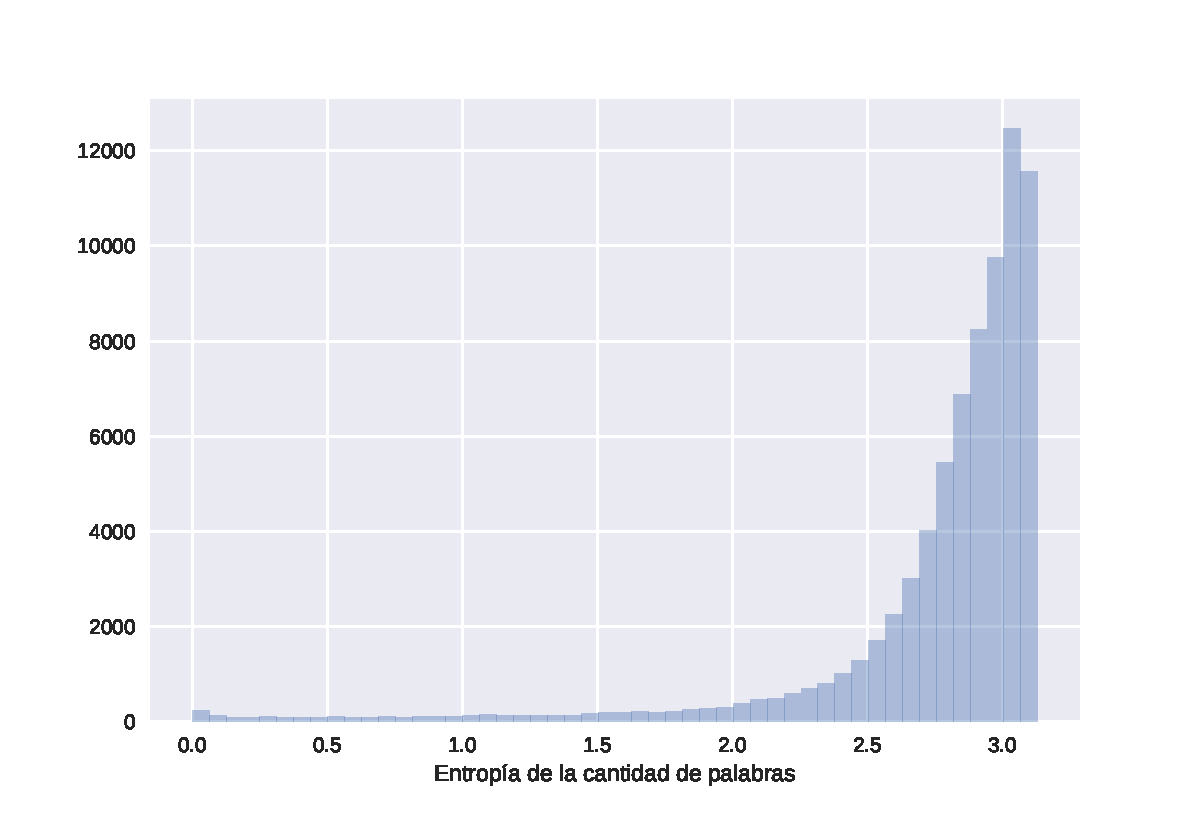
\includegraphics[width=1.0\textwidth]{./images/DistribucionEntropia.pdf}
\caption{Entropía de las Palabras} 
\label{fig:entropiaPalabras} 
\end{figure}

En el gráfico \ref{fig:entropiaPalabras} podemos ver que la mayor parte de las palabras tienen un valor de entropía entre 2.5 y 3. Esto quiere decir que hay un gran conjunto de palabras que tiene una cantidad de ocurrencias relativamente uniforme a lo largo de todas las provincias. Sin embargo hay otro conjunto de palabras que tienen una entropía menor a 2, la cual podemos considerar como baja. Estas útlimas palabras serán las que tienen mayor interés debido a que tienen una variación marcada en cuanto a su utilización en las distintas regiones.

Sin embargo, ver solamente la entropía de las palabras nos puede generar la detección de palabras que no son de interés, ya sea porque no ocurren una cantidad significativa o porque la variación de las ocurrencias en las distintas provincias se debe solamente a pocos usuarios que la utilizan mucho. Es por esto que también se calculó la entropía teniendo como variable la cantidad de personas que utilizaron cierto término en una determinada provincia.

\subsection{Valor de la información}
\label{sub:ValorDeLaInformacion}
En el gráfico \ref{fig:infoValue} se muestra una clara relación entre la cantidad de ocurrencias que tiene una palabra y su valor de la información, indicado por el color que tiene. A su vez, se nota que el valor de la información suele ser mayor a médida que el valor de la entropía es menor. Esto no siempre es el caso debido a que hay palabras que tiene una entropía de palabras baja, pero sin embargo la entropía de personas es alta logrando que el valor de la información sea bajo.

\begin{figure}[ht]
\centering
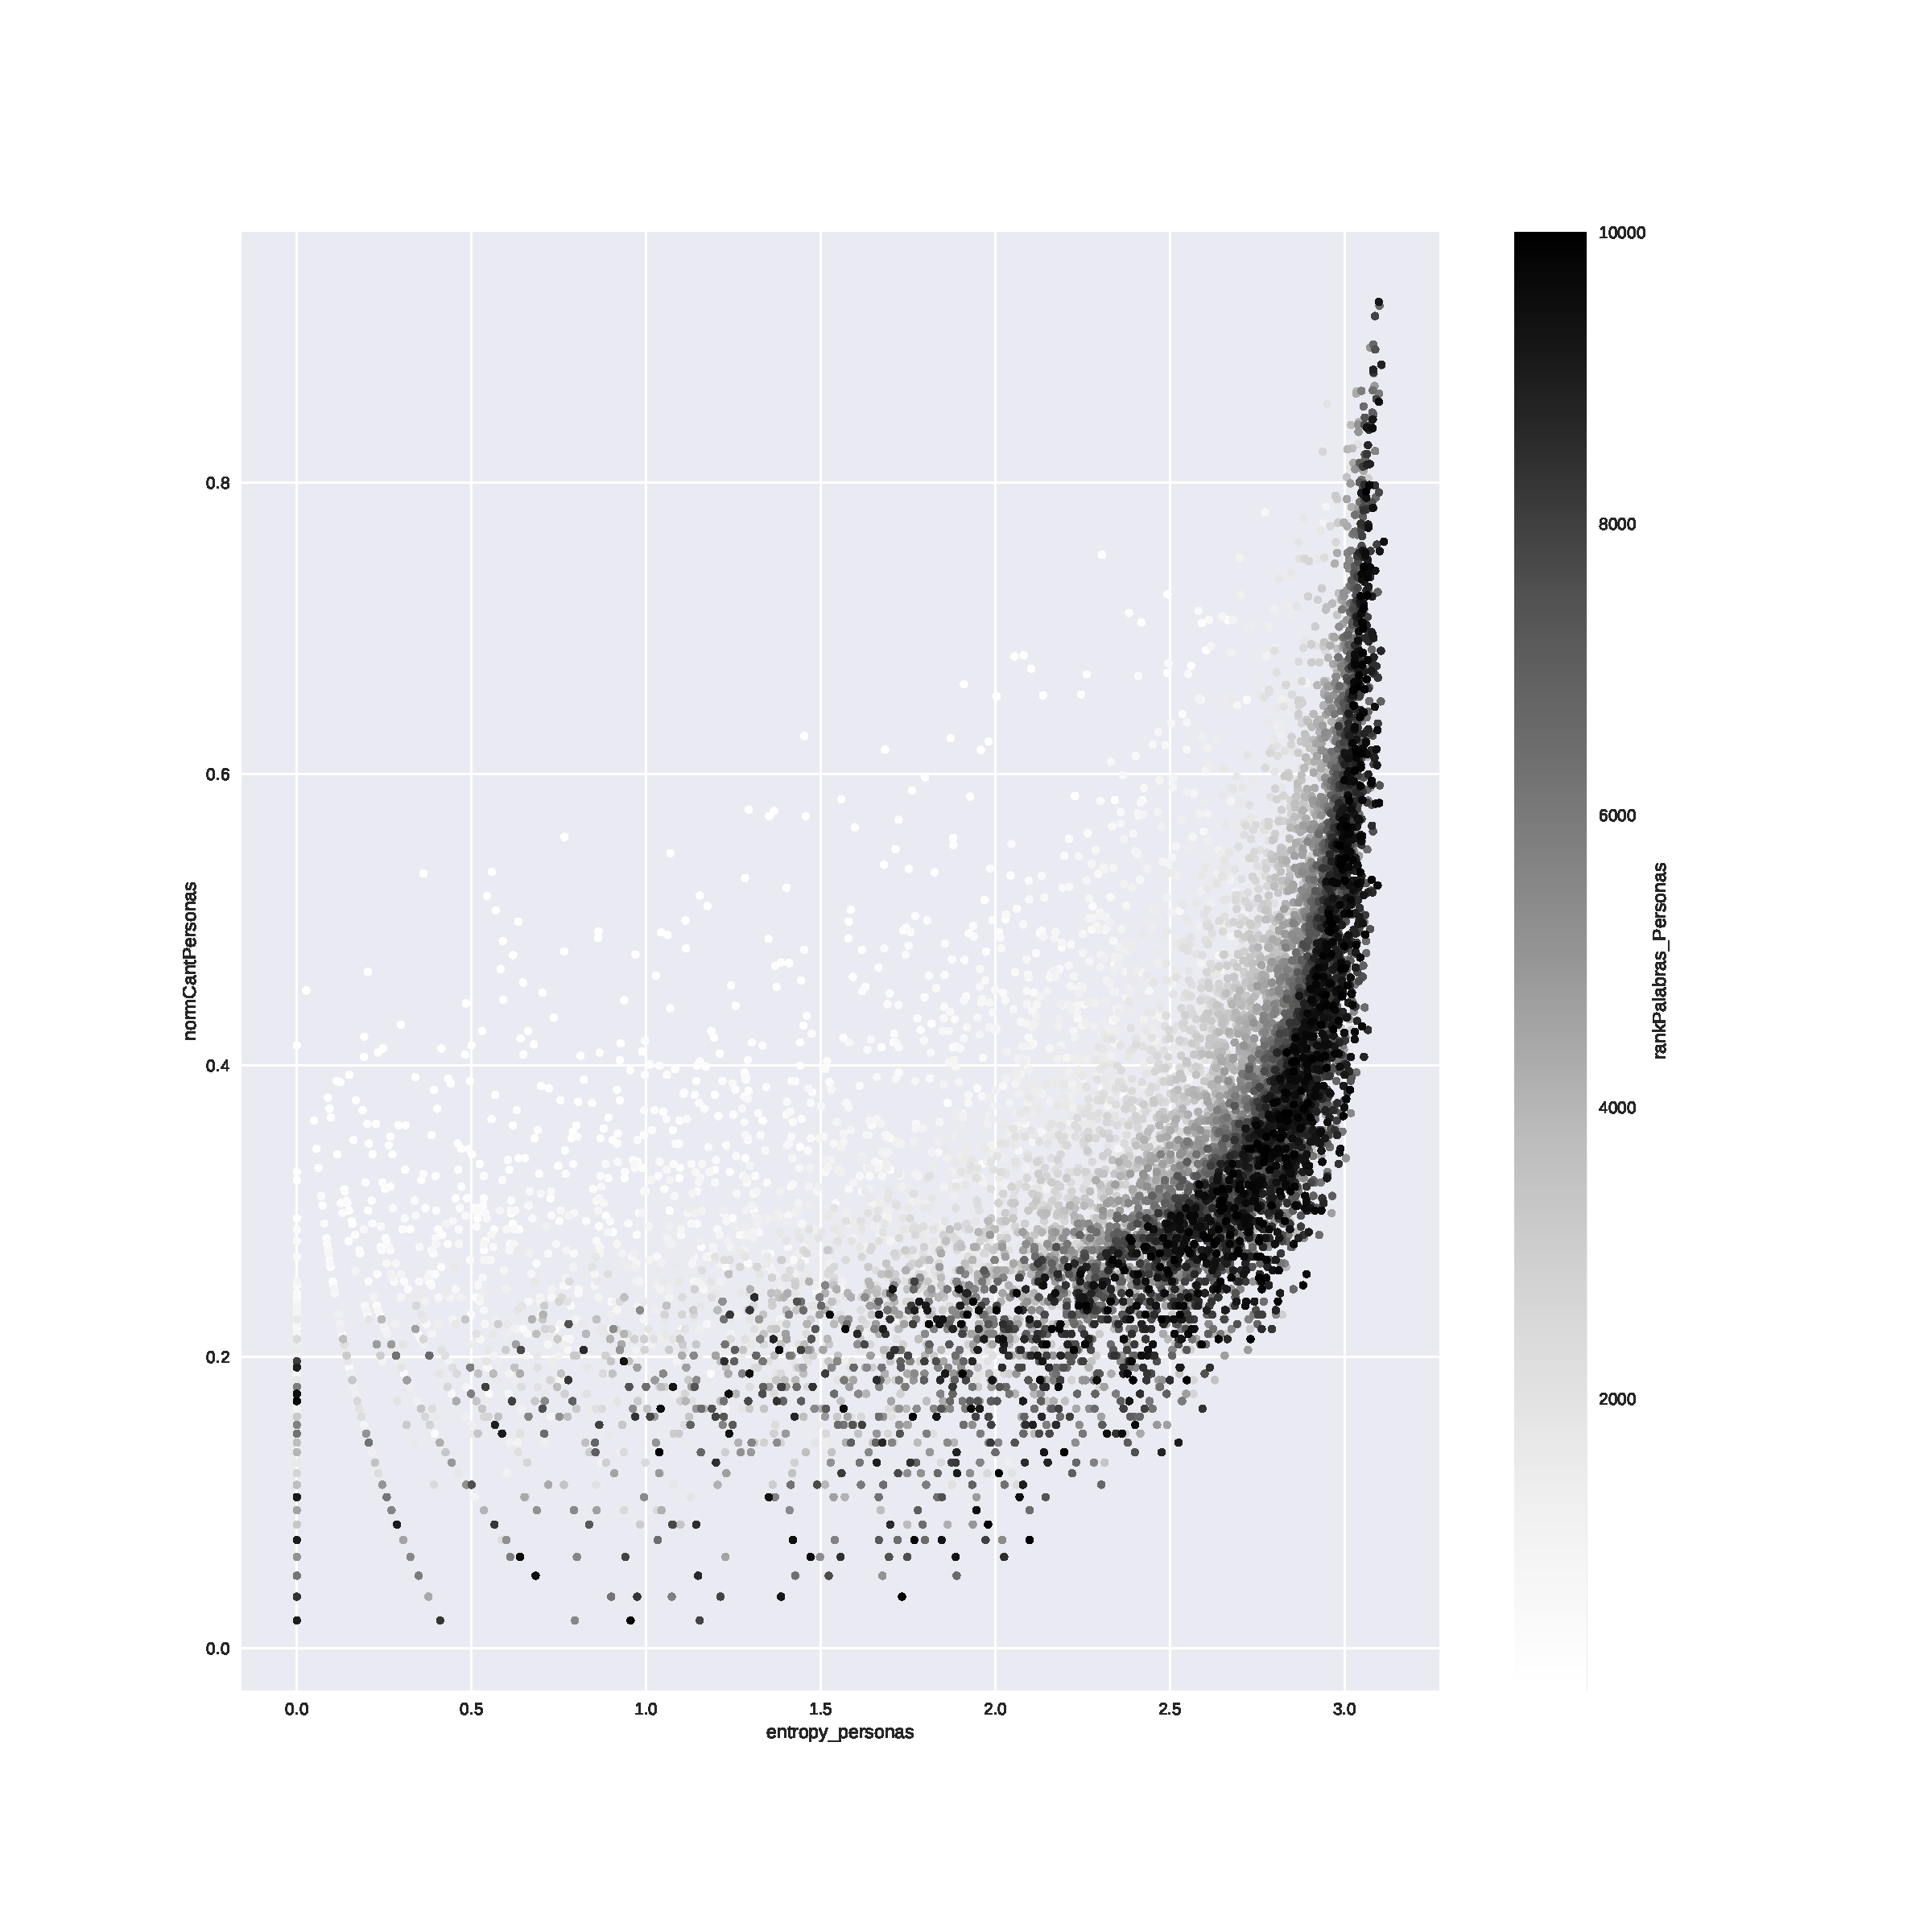
\includegraphics[width=1.0\textwidth]{./images/entropiaPersonasxNormCantPersonas.pdf}
\caption{Entropía de las Palabras} 
\label{fig:infoValue} 
\end{figure}

A continuación se puede ver el valor de la información según la posición en la que se encuentra en el listado ordenado por la misma.

\begin{figure}[!ht]\centering
   \begin{minipage}{0.49\textwidth}
    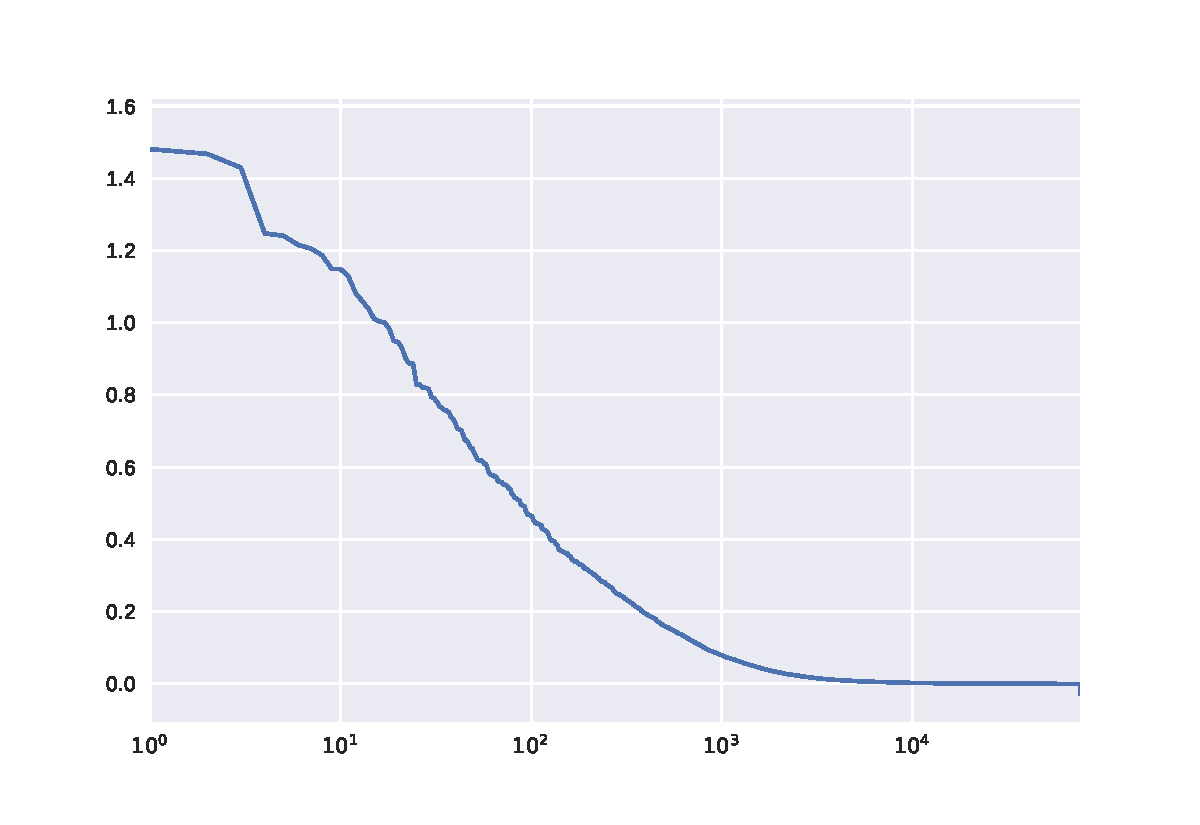
\includegraphics[width=\linewidth]{./images/ivaluesLog.pdf}
    \caption{Valor de la información} 
    \label{fig:ivalue}
   \end{minipage}
   \begin {minipage}{0.49\textwidth}
    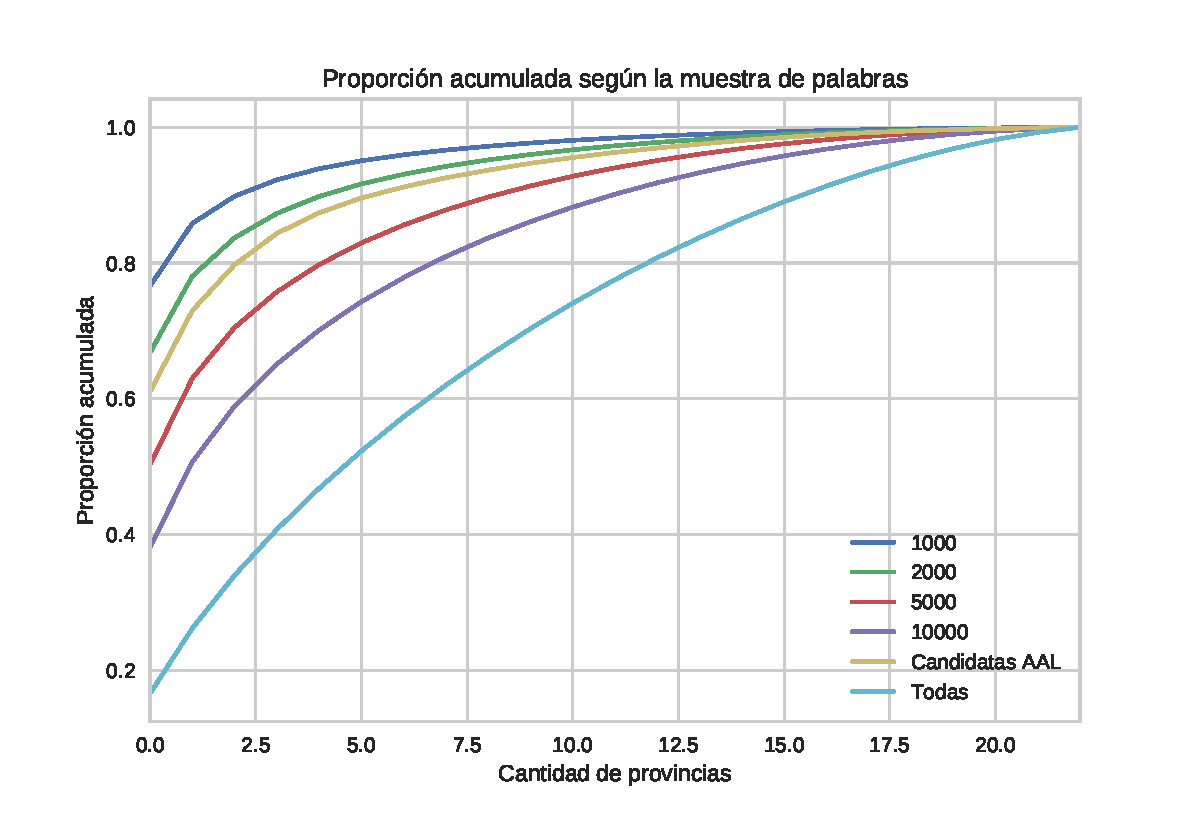
\includegraphics[width=\linewidth]{./images/PropAcum.pdf}
    \caption{Proporción acumulada según la muestra de palabras} 
    \label{fig:propAcum} 
   \end{minipage}
\end{figure}



\subsection{Proporción de ocurrencias} % (fold)
\label{sub:proporcionDeOcurrencias}


En la figura \ref{fig:propAcum} muestra la proporción acumulada de las palabras. Para esto, se ordenó para cada palabra las provincias según la cantidad de ocurrencias. Es notable la diferencia de proporciones acumuladas según la muestra de palabras. Solamente con una provincia para cada palabra ya se puede cubrir, en promedio, el 76\% del total de ocurrencias sobre las mil palabras con mayor valor de la información.

En el gráfico \ref{fig:propAcum5000} se observa la variación del cubrimiento de ocurrencias a médida que se aumenta la cantidad de provincias. 


\begin{figure}[h]
\centering
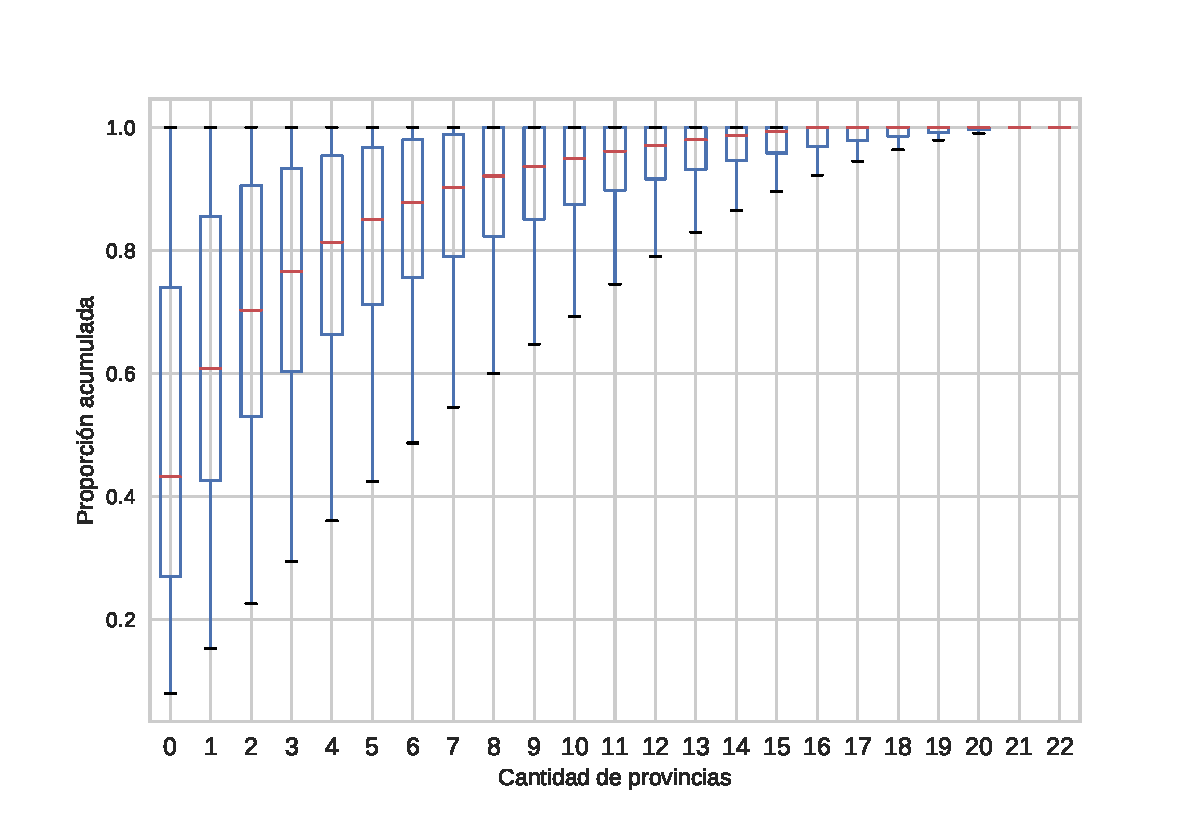
\includegraphics[width=0.5\textwidth]{./images/PropAcum5000.pdf}
\caption{Proporciones Acumuladas} 
\label{fig:propAcum5000} 
\end{figure}

\subsection{Palabras candidatas} % (fold)
\label{sub:palabras_candidatas}
Para buscar las palabras candidatas a tener contrastes significativos en cuanto a la cantidad de ocurrencias en distintas provincias, elegimos el conjunto de las primeras 
diez mil (10000) palabras con valor de la información más altas. El número 10000 surgió de ver la distribución de los valores de la información. Cómo se puede ver en 
el gráfico \ref{fig:ivalue} hay una caída pronunciada de la métrica y a partir de la palabra cuya posición es 4000 se ve que empieza a establizarse y los valores son 
muy cercanos a 0. Es por esto que nos pareción razonable dar un márgen de 10000 palabras para seleccionar las palabras con contrastes significativos.

Como era de esperar las ciudades y provincias son palabras que ocurren mayormente en las provinicias que estas indican. Es por esto que tienen una gran variación en 
la cantidad de ocurrencias en las distintas provincias, lo que genera un valor alto en la métrica de valor de la información. Para detectar las palabras que tienen 
mayor interés lingüistico buscamnos un conjunto de datos con los nombres de las localidades y departamentos de la República Argentina de modo tal que podamos filtrar 
los lugares del listado original.


\subsection{Regiones de palabras} % (fold)
\label{sub:regiones_de_palabras}

Una vez que calculamos las regiones que cubren un umbral para cada palabra, nos propusimos analizar cuales son las más frecuentes. Para eso generamos una lista con los conjuntos de provincias cuya cantidad sea menor o igual a 6 y los ordenamos según su frecuencia. A continuación se puede ver los primeros conjuntos de provincias obtenidos a partir de los primeras 5000 palabras más contrastivas de acuerdo al valor de la información:

\begin{table}[]
\centering
\label{tab:regiones}
\begin{tabular}{|c|c|}
\hline
Conjunto de provincias                                 & Cantidad de Palabras  \\ \hline
(Jujuy,Salta)                                          & 24          \\
(Mendoza, San Juan)                                    & 19          \\
(Neuquén, Río Negro)                                   & 18          \\
(Corrientes, Misiones)                                 & 16          \\
(Chaco, Corrientes, Formosa)                           & 16          \\
(Chaco, Corrientes)                                    & 16          \\
(chubut, Santa Cruz)                                   & 13          \\
(Catamarca, La Rioja)                                  & 12          \\
(Santa Cruz, Tierra del Fuego)                         & 12          \\
(Corrientes, Entre Ríos, Formosa, La Rioja, Misiones)  & 12          \\  %La Rioja está de más
(Formosa, Misiones)                                    & 12          \\
(Corrientes, Formosa, Misiones)                        & 12          \\
(Córdoba, La Rioja)                                    & 11          \\
(Catamarca, Salta, Santiago del Estero, Tucumán)       & 11          \\
(Catamarca, Jujuy, La Rioja, Salta, Santiago del Estero, Tucumán) & 10          \\
(Chaco, Corrientes, Misiones)                          & 10          \\
(Chaco, Corrientes, Formosa, Misiones)                 & 9           \\
(Catamarca, Santiago del Estero, Tucumán)              & 9           \\
(Catamarca, Tucumán)                                   & 9           \\
(Salta, Tucumán)                                       & 8           \\
(Catamarca, Jujuy, Salta, Santiago del Estero, Tucumán)& 8           \\
(Neuquén, San Juan)                                    & 7           \\ %no son contiguas pero están cercanas
(chubut, Santa Cruz, Tierra del Fuego)                 & 7           \\
(Buenos Aires, lapampa)                                & 7           \\
(Salta, Santiago del Estero, Tucumán)                  & 7           \\
(Buenos Aires, lapampa, Río Negro)                     & 6           \\
(Corrientes, Formosa)                                  & 6           \\
(Catamarca, Jujuy, Salta, Tucumán)                     & 6           \\
(Chaco, Corrientes, Entre Ríos, Formosa, Misiones)     & 6           \\
(Catamarca, Santiago del Estero)                       & 6           \\
\hline
\end{tabular}
\caption{Indica cuantas palabras tienen un cubrimiento del 80\% de sus ocurrencias en cada conjunto de provincias a partir de las 5000 palabras más contrastivas (de acuerdo al valor de la información).}
\end{table}

De la tabla \ref{tab:regiones} podemos destacar que la mayoría de las regiones son compuestas por provincias contiguas.

\begin{table}[]
\centering
{%
\begin{tabular}{|c|c|c|c|}
\hline
\multicolumn{4}{|c|}{Conjunto de Provincias} \\ \hline
\hline
Salta-Jujuy & Mendoza-San Juan & Chubut-Santa Cruz-T. Del Fuego & Chaco-Corrientes-Formosa   \\ \hline
tribuno     & mza              & austral                        & anga                       \\
salteño     & zonda            & chilote                        & teresss                    \\
orán        & secamente        & calafa                         & músicas                    \\
tartagal    & sanjuaninos      & chilota                        & argela                     \\
salteña     & sanjuanino       & palmaso                        & angaaa                     \\
martearena  & asar             & vueltines                      & olo                        \\
oran        & tomba            & riviera                        & cuchale                    \\
yuto        & queras           &                                & corrientesss               \\
purmamarca  & traica           &                                & angá                       \\
yutos       & sopaipillas      &                                & cts                        \\
gorriti     & ardente          &                                & correntinas                \\
quijano     & secamentes       &                                & iburrr                     \\
tabacal     & jáchal           &                                & cheraa                     \\
desentierro & virreina         &                                & cheraá                     \\
huaico      & tombaaa          &                                & bofill                     \\
pichanal    & mansooo          &                                & receppp                    \\
diableros   & tombino          &                                &                            \\
bandy       & parisi           &                                &                            \\
aramayo     & asadaaa          &                                &                            \\
ñaño        &                  &                                &                            \\
colque      &                  &                                &                            \\
urkupiña    &                  &                                &                            \\
juy         &                  &                                &                            \\
guachipas   &                  &                                &                            \\ \hline
\end{tabular}%
}
\caption{Palabras cubiertas sobre el 80\% de las ocurrencias totales por el conjunto de provincias a partir de las 5000 palabras más contrastivas (de acuerdo al valor de la información).}
\label{tab:palabrasRegiones}
\end{table}


\subsection{Validación}
ACA VA LOS RESULTADOS DEL TEST HIPERGEOMETRICO EN EL CONJUNTO DE VALIDACIÓN

\subsection{Ruido}
\label{ssub:ruido}

Cuando vimos las palabras con mayor valor de la información, nos dimos cuenta de que algunas palabras de la provincia de La Rioja eran provenientes de España. Analizando la causa de este ruido, nos dimos cuenta que la API de Twitter no realiza las búsquedas localizadas como uno esperaría. En particular, no solo se fija en los tweets geolocalizados, sino que también hace una búsqueda inversa a través de los nombres de las ciudades que tienen esa coordenada. Específicamente La Rioja es una provincia Argentina, como así también una provincia de España. Es por eso que al hacer búsquedas con las coordenadas de ciudades de La Rioja en Argentina, tuvimos resultados de tweets de España. A pesar de que los tweets no fueron escritos en Argentina, consideramos que su cantidad no es lo suficientemente grande como para tener resultados incorrectos.

% Histograma de la distribucion del valor de la información

